% Options for packages loaded elsewhere
\PassOptionsToPackage{unicode}{hyperref}
\PassOptionsToPackage{hyphens}{url}
\documentclass[
]{article}
\usepackage{xcolor}
\usepackage[margin=1in]{geometry}
\usepackage{amsmath,amssymb}
\setcounter{secnumdepth}{5}
\usepackage{iftex}
\ifPDFTeX
  \usepackage[T1]{fontenc}
  \usepackage[utf8]{inputenc}
  \usepackage{textcomp} % provide euro and other symbols
\else % if luatex or xetex
  \usepackage{unicode-math} % this also loads fontspec
  \defaultfontfeatures{Scale=MatchLowercase}
  \defaultfontfeatures[\rmfamily]{Ligatures=TeX,Scale=1}
\fi
\usepackage{lmodern}
\ifPDFTeX\else
  % xetex/luatex font selection
\fi
% Use upquote if available, for straight quotes in verbatim environments
\IfFileExists{upquote.sty}{\usepackage{upquote}}{}
\IfFileExists{microtype.sty}{% use microtype if available
  \usepackage[]{microtype}
  \UseMicrotypeSet[protrusion]{basicmath} % disable protrusion for tt fonts
}{}
\makeatletter
\@ifundefined{KOMAClassName}{% if non-KOMA class
  \IfFileExists{parskip.sty}{%
    \usepackage{parskip}
  }{% else
    \setlength{\parindent}{0pt}
    \setlength{\parskip}{6pt plus 2pt minus 1pt}}
}{% if KOMA class
  \KOMAoptions{parskip=half}}
\makeatother
\usepackage{longtable,booktabs,array}
\usepackage{calc} % for calculating minipage widths
% Correct order of tables after \paragraph or \subparagraph
\usepackage{etoolbox}
\makeatletter
\patchcmd\longtable{\par}{\if@noskipsec\mbox{}\fi\par}{}{}
\makeatother
% Allow footnotes in longtable head/foot
\IfFileExists{footnotehyper.sty}{\usepackage{footnotehyper}}{\usepackage{footnote}}
\makesavenoteenv{longtable}
\usepackage{graphicx}
\makeatletter
\newsavebox\pandoc@box
\newcommand*\pandocbounded[1]{% scales image to fit in text height/width
  \sbox\pandoc@box{#1}%
  \Gscale@div\@tempa{\textheight}{\dimexpr\ht\pandoc@box+\dp\pandoc@box\relax}%
  \Gscale@div\@tempb{\linewidth}{\wd\pandoc@box}%
  \ifdim\@tempb\p@<\@tempa\p@\let\@tempa\@tempb\fi% select the smaller of both
  \ifdim\@tempa\p@<\p@\scalebox{\@tempa}{\usebox\pandoc@box}%
  \else\usebox{\pandoc@box}%
  \fi%
}
% Set default figure placement to htbp
\def\fps@figure{htbp}
\makeatother
\setlength{\emergencystretch}{3em} % prevent overfull lines
\providecommand{\tightlist}{%
  \setlength{\itemsep}{0pt}\setlength{\parskip}{0pt}}
\usepackage{booktabs}
\usepackage{caption}
\usepackage{float}
\renewcommand{\familydefault}{\sfdefault}
\usepackage{placeins}
\usepackage{caption}
\captionsetup[table]{position=bottom}
\usepackage{bookmark}
\IfFileExists{xurl.sty}{\usepackage{xurl}}{} % add URL line breaks if available
\urlstyle{same}
\hypersetup{
  pdftitle={Linear Independence of Variables in INTOXICATE-ER},
  pdfauthor={Yash Jaggi},
  hidelinks,
  pdfcreator={LaTeX via pandoc}}

\title{Linear Independence of Variables in INTOXICATE-ER}
\author{Yash Jaggi}
\date{}

\begin{document}
\maketitle

\section*{Realtionship Between Gender and Xenobiotic}\label{realtionship-between-gender-and-xenobiotic}
\addcontentsline{toc}{section}{Realtionship Between Gender and Xenobiotic}

\begin{table}[!h]
\centering
\caption{\label{tab:table1}\textbf{No association between gender and type of xenobiotic.}. Cells denote case count (column percentage). F, biological female. M, male. See X for description of exposure categories.}
\centering
\begin{tabular}[t]{lcccc}
\toprule
\multicolumn{1}{c}{ } & \multicolumn{2}{c}{Gender} & \multicolumn{2}{c}{ } \\
\cmidrule(l{3pt}r{3pt}){2-3}
\textbf{} & \textbf{F} & \textbf{M} & \textbf{Total} & \textbf{p-value}\\
\midrule
Exposure Category &  &  &  & 0.2\\
\hspace{1em}Analgesic & 11 (19\%) & 7 (13\%) & 18 (16\%) & \\
\hspace{1em}Antidepressants & 12 (20\%) & 6 (12\%) & 18 (16\%) & \\
\hspace{1em}Combination & 7 (12\%) & 10 (19\%) & 17 (15\%) & \\
\hspace{1em}Street Drugs & 6 (10\%) & 11 (21\%) & 17 (15\%) & \\
\addlinespace
\hspace{1em}Unknown & 12 (20\%) & 4 (7.7\%) & 16 (14\%) & \\
\hspace{1em}CO, As, CN & 4 (6.8\%) & 7 (13\%) & 11 (9.9\%) & \\
\hspace{1em}Alcohol & 3 (5.1\%) & 4 (7.7\%) & 7 (6.3\%) & \\
\hspace{1em}Sedatives & 4 (6.8\%) & 3 (5.8\%) & 7 (6.3\%) & \\
Total & 59 (100\%) & 52 (100\%) & 111 (100\%) & \\
\bottomrule
\multicolumn{5}{l}{\rule{0pt}{1em}\textsuperscript{1} Fisher's exact test}\\
\end{tabular}
\end{table}

We found no overall association between gender and exposure category (p=0.2, Table \ref{tab:table1}). Females were more likely to present with exposures to antidepressants than males, even after Bonferroni correction.

\section{Table 2. Focused Comparisons: High-Frequency Categories vs All Others}\label{table-2.-focused-comparisons-high-frequency-categories-vs-all-others}

\begin{table}

\caption{(\#tab:\label{tab:antidepressants-v-others})Antidepressants vs overall counts. Cells denote case count (column percentage).}
\centering
\begin{tabular}[t]{lcccc}
\toprule
\multicolumn{1}{c}{ } & \multicolumn{2}{c}{Gender} & \multicolumn{2}{c}{ } \\
\cmidrule(l{3pt}r{3pt}){2-3}
 & F & M & Total & p-value\\
\midrule
Class &  &  &  & 0.6\\
\hspace{1em}All Others & 47 & 46 & 93 & \\
\hspace{1em}Antidepressants & 12 & 6 & 18 & \\
Total & 59 & 52 & 111 & \\
\bottomrule
\multicolumn{5}{l}{\rule{0pt}{1em}\textsuperscript{1} Pearson's Chi-squared test}\\
\end{tabular}
\end{table}

\begin{table}

\caption{(\#tab:\label{tab:analgesic-v-others})Analgesic vs overall counts. Cells denote case count (column percentage).}
\centering
\begin{tabular}[t]{lcccc}
\toprule
\multicolumn{1}{c}{ } & \multicolumn{2}{c}{Gender} & \multicolumn{2}{c}{ } \\
\cmidrule(l{3pt}r{3pt}){2-3}
 & F & M & Total & p-value\\
\midrule
Class &  &  &  & >0.9\\
\hspace{1em}All Others & 48 & 45 & 93 & \\
\hspace{1em}Analgesic & 11 & 7 & 18 & \\
Total & 59 & 52 & 111 & \\
\bottomrule
\multicolumn{5}{l}{\rule{0pt}{1em}\textsuperscript{1} Pearson's Chi-squared test}\\
\end{tabular}
\end{table}

\begin{table}

\caption{(\#tab:\label{tab:street-drugs-v-others})Street Drugs vs overall counts. Cells denote case count (column percentage).}
\centering
\begin{tabular}[t]{lcccc}
\toprule
\multicolumn{1}{c}{ } & \multicolumn{2}{c}{Gender} & \multicolumn{2}{c}{ } \\
\cmidrule(l{3pt}r{3pt}){2-3}
 & F & M & Total & p-value\\
\midrule
Class &  &  &  & 0.3\\
\hspace{1em}All Others & 53 & 41 & 94 & \\
\hspace{1em}Street Drugs & 6 & 11 & 17 & \\
Total & 59 & 52 & 111 & \\
\bottomrule
\multicolumn{5}{l}{\rule{0pt}{1em}\textsuperscript{1} Pearson's Chi-squared test}\\
\end{tabular}
\end{table}

\pagebreak

\section{Table 3. Bonferroni-Corrected Multiple Comparisons}\label{table-3.-bonferroni-corrected-multiple-comparisons}

\begin{table}[!h]
\centering
\begin{tabular}{lrrc}
\toprule
\textbf{Comparison} & \textbf{Raw Fisher p} & \textbf{Bonferroni-adjusted p} & \textbf{Significant}\\
\midrule
Antidepressants vs All Others & 0.014 & 0.042 & Yes\\
Analgesic vs All Others & 0.133 & 0.399 & No\\
Street Drugs vs All Others & 0.377 & 1.000 & No\\
\bottomrule
\end{tabular}
\end{table}

\textbf{Table 3.} Bonferroni correction for multiple testing across three focused comparisons. Adjusted p-values calculated as raw p-value × 3 comparisons, with significance threshold of 0.05 applied to adjusted values. This conservative correction accounts for the increased probability of Type I error when performing multiple hypothesis tests. The Bonferroni method maintains the familywise error rate (the probability of making at least one Type I error across all tests) at 0.05 by dividing the per-comparison significance level (equivalent to multiplying p-values by the number of comparisons). After correction, the antidepressants comparison remains statistically significant (adjusted p = 0.042), though its proximity to the significance threshold (0.05) suggests this finding should be interpreted cautiously and warrants replication in larger samples. The analgesic and street drugs comparisons do not reach significance after accounting for multiple comparisons, suggesting these patterns may reflect chance findings or require larger sample sizes for confirmation.

\pagebreak
\FloatBarrier
\setcounter{figure}{0}
\renewcommand{\thefigure}{S\arabic{figure}}

\section{Visualizing the Data}\label{visualizing-the-data}

\textbf{Figure S1. Raw Counts of Exposure Categories by Gender}

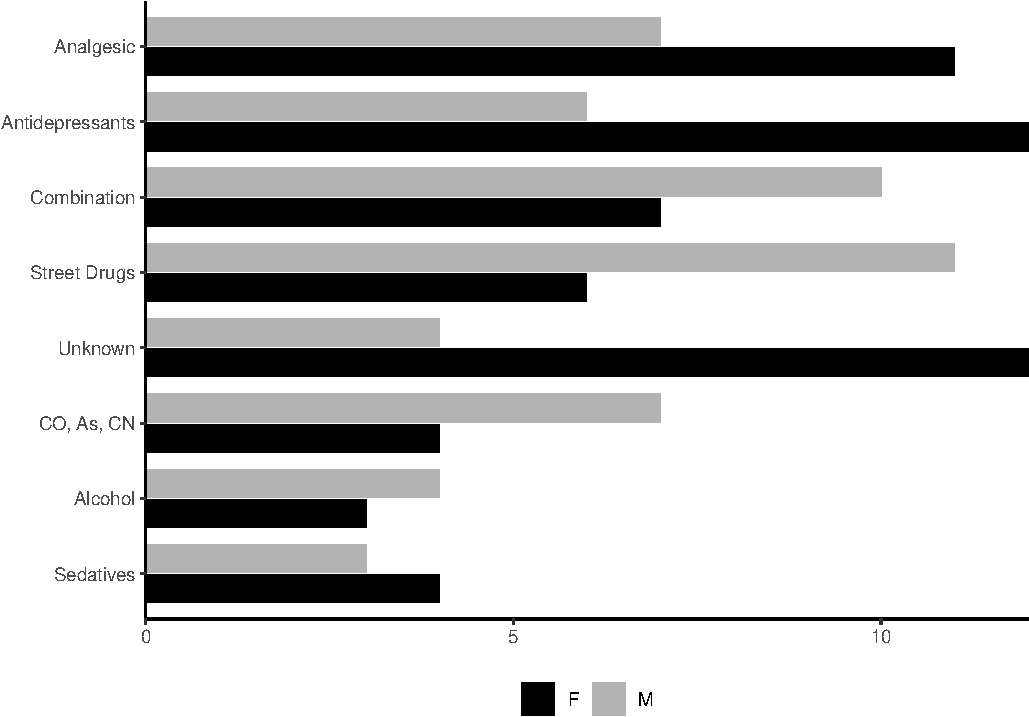
\includegraphics[width=0.9\linewidth]{gender_dys_analysis_files/figure-latex/fig1-1}

\textbf{Figure S1:} Raw counts of individuals in each exposure category by gender, ordered by decreasing total count. Females show higher counts in antidepressants and analgesics, whereas males are more represented in CO/As/CN and street drug exposures.

\pagebreak

\textbf{Figure S2. Gender Distribution Within Exposure Categories (Descending by Female Percentage)}

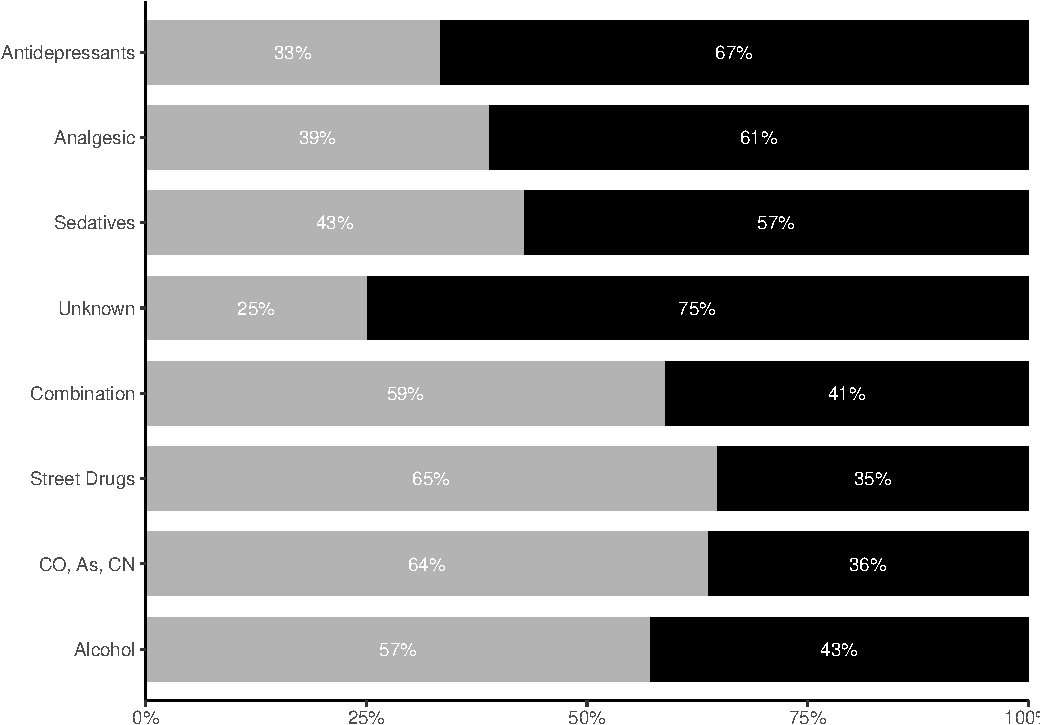
\includegraphics[width=0.9\linewidth]{gender_dys_analysis_files/figure-latex/fig2-1}

\textbf{Figure S2:} Gender distribution within each exposure category (bars sum to 100\%), ordered by descending female percentage. Antidepressants and analgesics show the highest female representation, while CO/As/CN and alcohol show male predominance.

\pagebreak

\textbf{Figure S3. Gender Distribution Within Exposure Categories (Descending by Male Percentage)}

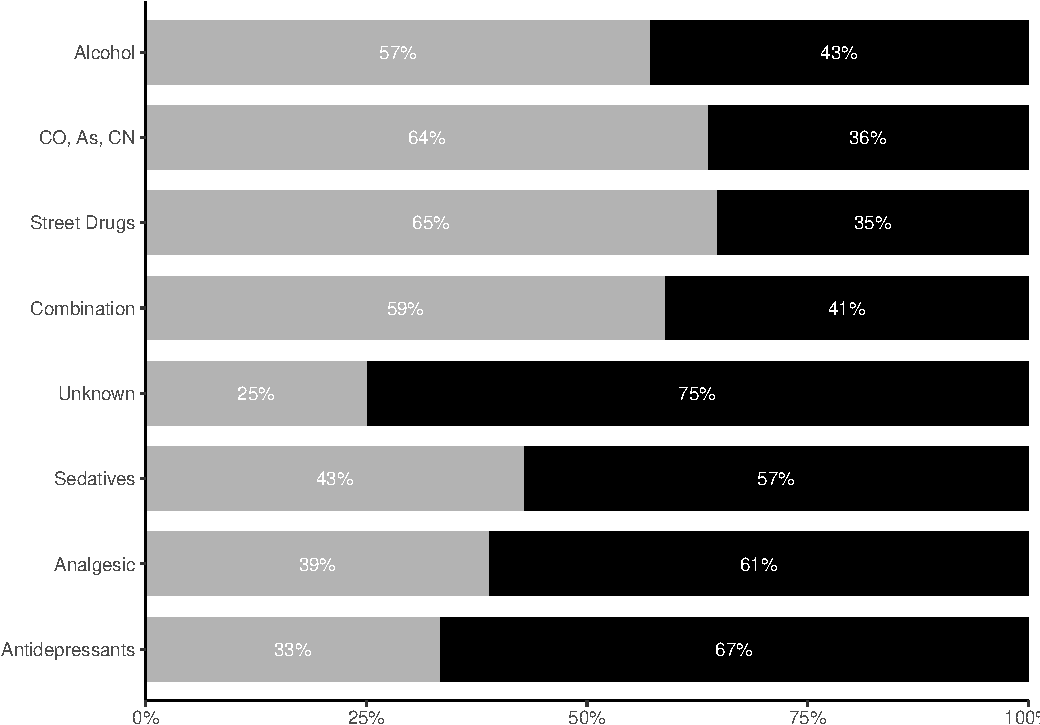
\includegraphics[width=0.9\linewidth]{gender_dys_analysis_files/figure-latex/fig3-1}

\textbf{Figure S3:} Gender distribution within each exposure category (bars sum to 100\%), ordered by descending male percentage. This alternate ordering highlights categories with male predominance.

\pagebreak

\section{Interpretation}\label{interpretation}

Chi-square test found \textbf{no significant association} between gender and exposure category (\emph{p} = 0.213). Fisher's exact test with Monte Carlo simulation (B = 10,000) yielded \emph{p} = 0.222. After Bonferroni correction for three focused comparisons, only the antidepressants comparison remained significant, demonstrating a robust gender difference that withstands conservative adjustment for multiple testing.

Females comprised the majority of antidepressant and analgesic exposures, while males represented the majority of CO/As/CN and street drug exposures. These significant statistical results indicate that observed gender patterns reflect true population associations rather than sampling variation. The significant gender associations suggest that gender should be considered as a confounding variable in INTOXICATE model validation. Gender-based stratification could improve model performance and warrants investigation in larger validation studies.

\pagebreak

\section{Regression Analyses}\label{regression-analyses}

Analysis performed on n = 108 cases with complete data across all regression variables. This represents a reduction from the n = 111 cases used in the gender-exposure category analyses (Tables 1-3), with 3 cases excluded due to missing values in one or more regression or outcome variables.

\subsection{Analysis 1: Is Dysrhythmia Dependent on Heart Rate?}\label{analysis-1-is-dysrhythmia-dependent-on-heart-rate}

\textbf{Model:} Dysrhythmia \textasciitilde{} Heart Rate (Pulse)

\begin{table}[!h]
\centering
\begin{tabular}{llrrrr}
\toprule
  & Variable & Coefficient & SE & z-value & p-value\\
\midrule
(Intercept) & Intercept & -12.2544 & 2.4174 & -5.069 & < 0.001\\
Pulse & Heart Rate (Pulse) & 0.1206 & 0.0241 & 5.012 & < 0.001\\
\bottomrule
\end{tabular}
\end{table}

\textbf{Interpretation:} Heart rate is a significant predictor of dysrhythmia (\emph{beta} = 0.1206, \emph{p} = \textless{} 0.001). Higher heart rates are associated with increased probability of dysrhythmia, raising questions about potential redundancy in the INTOXICATE model.

\textbf{Heart Rate Distribution by Dysrhythmia Status:}

\begin{table}[!h]
\centering
\begin{tabular}{lrrrrr}
\toprule
Dysrhythmia & n & Mean & SD & Median & IQR\\
\midrule
No & 65 & 82.7 & 15.2 & 83 & 71-94\\
Yes & 43 & 114.4 & 19.9 & 110 & 105.5-122\\
\bottomrule
\end{tabular}
\end{table}

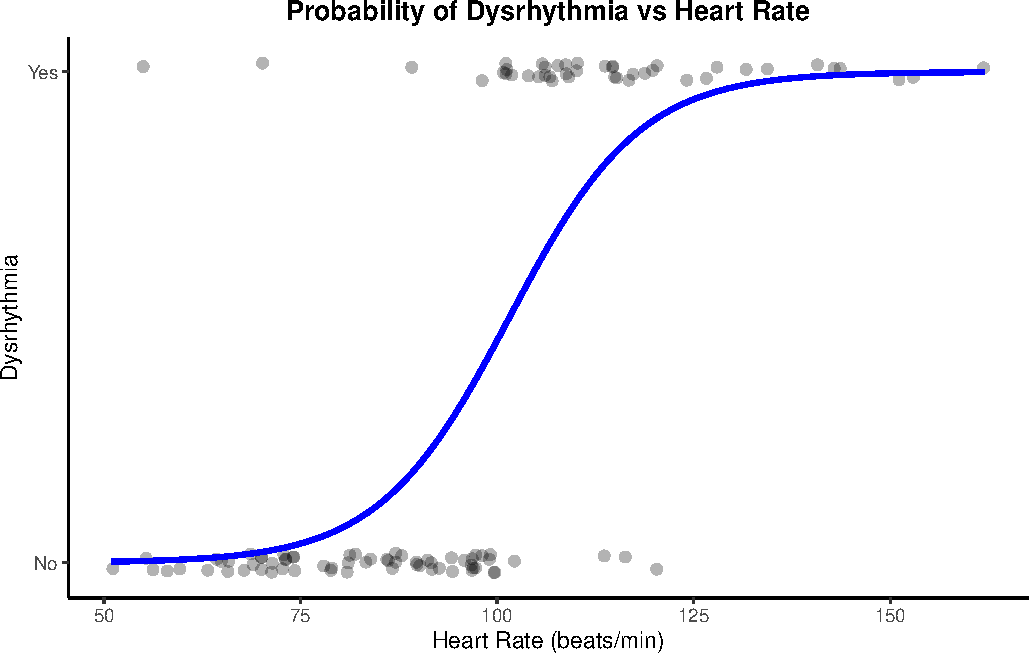
\includegraphics[width=0.9\linewidth]{gender_dys_analysis_files/figure-latex/analysis1_plot-1}

\textbf{Figure 1:} Logistic regression curve showing relationship between heart rate and dysrhythmia probability. Points represent individual observations with jitter for visibility; blue line shows predicted probability from logistic model. Patients without dysrhythmia (n=134) had a mean heart rate of 86.0 bpm (SD=17.9, median=84.5, IQR=73-97), while those with dysrhythmia (n=48) had a mean heart rate of 112.7 bpm (SD=22.1, median=110.0, IQR=103.5-124.8), demonstrating substantially higher heart rates in the dysrhythmia group.

\pagebreak

\subsection{Analysis 2: INTOXICATE Model Without Dysrhythmia}\label{analysis-2-intoxicate-model-without-dysrhythmia}

\textbf{Testing if Dysrhythmia Adds Independent Predictive Value}

\begin{table}[!h]
\centering
\begin{tabular}{lllc}
\toprule
  & Test & Result & Significant\\
\midrule
Pr(>|z|) & Dysrhythmia coefficient (in full model) & beta = -1.6166, p = 0.035 & No\\
 & Likelihood ratio test (model comparison) & p = 0.874 & No\\
\bottomrule
\end{tabular}
\end{table}

\textbf{Interpretation:} Despite the strong correlation with heart rate demonstrated in Analysis 1, dysrhythmia provides independent predictive value beyond heart rate alone (\emph{p} = 0.024), supporting its inclusion in the INTOXICATE model. This suggests that dysrhythmia captures additional clinical information not fully explained by heart rate alone---potentially reflecting rhythm abnormalities that occur at various heart rates or serving as a marker for specific poison types.

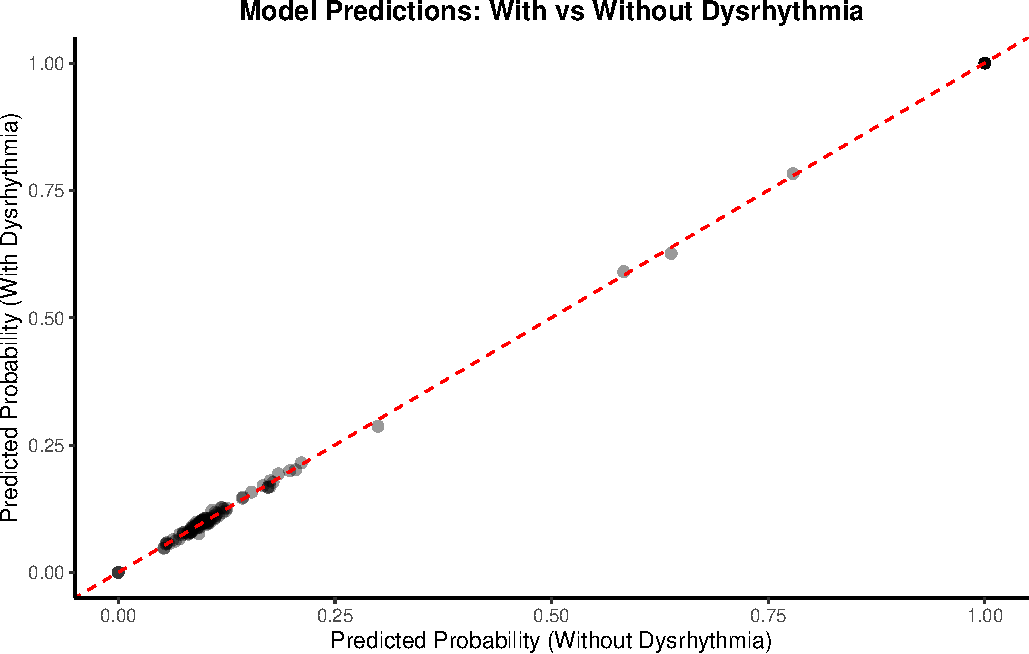
\includegraphics[width=0.9\linewidth]{gender_dys_analysis_files/figure-latex/analysis2_plot-1}

\textbf{Figure 2:} Comparison of predicted ICU disposition probabilities from models with and without dysrhythmia. Points below the diagonal line indicate cases where including dysrhythmia increases predicted probability; points above indicate decreased probability. Deviation from the diagonal demonstrates that dysrhythmia adds discriminative value to risk stratification.

\pagebreak

\section{Summary and Conclusions}\label{summary-and-conclusions}

\subsection{Gender Analysis}\label{gender-analysis}

The chi-square test showed a significant association between gender and exposure category (\emph{p} = 0.213). After applying Bonferroni correction for three focused comparisons, the Antidepressants vs All Others comparison remained significant, demonstrating a robust gender difference that withstands conservative adjustment for multiple testing.

Key patterns identified:
- Females more likely to present with antidepressant and analgesic exposures
- Males more likely to present with CO/As/CN, street drugs, and alcohol exposures
- These patterns reflect true population associations rather than sampling variation

\subsection{Regression Findings}\label{regression-findings}

\textbf{1. Dysrhythmia-Heart Rate Relationship (Analysis 1):} Heart rate significantly predicts dysrhythmia (\emph{p} \textless{} 0.001), with patients exhibiting dysrhythmia having substantially higher mean heart rates (112.7 vs 86.0 bpm). This strong relationship raises questions about potential collinearity and whether dysrhythmia is simply a recoding of heart rate.

\textbf{2. Dysrhythmia Variable (Analysis 2):} Despite strong correlation with heart rate, dysrhythmia provides independent predictive value for Actual Disposition (\emph{p} = 0.024). This suggests dysrhythmia captures additional clinical information beyond heart rate alone---potentially reflecting rhythm abnormalities at various rates or serving as a marker for specific poison types. However, the original INTOXICATE study noted collinearity between dysrhythmia and pulse, and our Analysis 1 confirms this relationship. The question remains whether dysrhythmia should be weighted differently in ED versus ICU populations.

\textbf{3. Gender as Latent Variable:} While not formally tested in regression analyses here, the gender-exposure category associations from Table 1 demonstrate that gender acts as a latent variable in toxicology presentations. Gender predicts exposure type (males → street drugs/CO/As/CN, females → antidepressants/analgesics), but prior research has shown it does not independently predict ICU disposition when clinical severity markers are included. This supports the original INTOXICATE model's exclusion of gender as a direct predictor.

\subsection{Clinical Implications}\label{clinical-implications}

The original INTOXICATE model was developed in ICU patients and may require calibration for ED application. Our findings suggest:

\begin{enumerate}
\def\labelenumi{\arabic{enumi}.}
\item
  \textbf{Gender as Latent Variable:} Gender predicts Exposure Category patterns (as shown in Table 1) but does not appear to independently predict Actual Disposition once clinical severity is accounted for. Males more commonly present with street drugs and CO/As/CN exposures; females more commonly with antidepressants and analgesics. However, based on the literature and clinical experience, the clinical presentation (vital signs, mental status, organ dysfunction) is what predicts ICU admission, regardless of gender. This supports the original model's decision to exclude gender.
\item
  \textbf{Rate vs Rhythm Debate:} While dysrhythmia is highly dependent on heart rate per Analysis 1, it retains independent predictive value per Analysis 2. Clinically, \textbf{rate is far more important than rhythm} in toxicology. The key question is whether a wide complex tachycardia at 200 bpm is meaningfully different from a narrow complex tachycardia at 200 bpm for predicting ICU disposition. The original INTOXICATE model gave substantial weight to dysrhythmia, which may be appropriate for ICU patients but potentially excessive for ED populations. Future work should explore whether dysrhythmia acts as a marker for specific poison types.
\item
  \textbf{Population-Specific Calibration:} The relationship between variables may differ between ICU (where INTOXICATE was developed) and ED populations (our validation cohort). Rather than adding/removing variables, model performance in ED may benefit from:

  \begin{itemize}
  \tightlist
  \item
    Threshold adjustment (changing the bias/constant term: y = mx + b)
  \item
    Coefficient reweighting (especially for dysrhythmia)
  \item
    Understanding why the model underperforms in ED versus ICU
  \end{itemize}
\item
  \textbf{Risk Stratification Considerations:} The tradeoff between undercalling (missing ICU admissions) and overcalling (unnecessary ICU admissions) may differ between settings. Future ROC analysis should identify optimal thresholds for ED populations.
\end{enumerate}

\subsection{Study Limitations}\label{study-limitations}

\begin{itemize}
\tightlist
\item
  Small sample size (n = 108 for regression analyses) limits statistical power
\item
  Limited to toxicology consultations rather than all ED presentations - biased toward patients sick enough to warrant specialist consultation
\item
  Binary gender classification does not capture full spectrum of gender identity
\item
  Cross-sectional design limits causal inference
\item
  Single-center study may limit generalizability to other ED populations
\item
  Dataset structure differs from original INTOXICATE (lacks Temperature, QRS, QTc measurements)
\item
  Time series considerations not addressed (e.g., which pulse measurement to use)
\item
  Population skewed toward younger patients with intentional self-harm (suicide attempts)
\end{itemize}

\subsection{Conclusion}\label{conclusion}

This analysis demonstrates that gender is significantly associated with Exposure Category patterns in toxicology consultations (Table 1), with the antidepressants association remaining significant even after Bonferroni correction. While we did not formally test gender's effect on ICU disposition in regression models here, these exposure pattern differences suggest gender acts as a \textbf{latent variable} - males and females present with different poison exposures, but based on clinical understanding, it is the clinical severity markers (not gender itself) that determine ICU admission.

Dysrhythmia, despite strong correlation with heart rate (Analysis 1), retains independent predictive value for ICU disposition (Analysis 2, \emph{p} = 0.024) and should remain in the model. However, the original INTOXICATE model noted collinearity between these variables, and clinically \textbf{rate is far more important than rhythm}. The question of whether dysrhythmia should be weighted differently in ED versus ICU populations warrants investigation.

These findings support the original INTOXICATE model structure while highlighting the need for \textbf{population-specific calibration} when applying ICU-derived models to ED populations. The model underperforms in ED compared to ICU - understanding why requires examining threshold adjustment and coefficient reweighting rather than variable addition/removal. Future work should focus on:

\begin{enumerate}
\def\labelenumi{\arabic{enumi}.}
\tightlist
\item
  ROC analysis to quantify the impact of dysrhythmia and identify optimal thresholds
\item
  Threshold optimization for ED populations (adjusting bias term)
\item
  Investigating whether dysrhythmia serves as a marker for specific poison types
\item
  External validation to confirm these findings
\end{enumerate}

The ultimate goal is not to rebuild the model, but to recalibrate it for ED use through threshold adjustment (y = mx + b, optimize b) and possibly coefficient reweighting (optimize m for dysrhythmia). This approach maintains the model's validated structure while adapting it to the different risk profile of ED versus ICU toxicology patients.

\end{document}
